\chapter{Basic modification strategy}
\label{s:basic-modification-strategy}
\label{s:last-strategy}
\is{language strategy!for colour!basic modification strategy}
\is{basic modification strategy|see{language strategy}}

Next to the basic colour strategy, most languages allow to
specify certain aspects of a colour through the use of modifiers. In
English and Chinese, the use of ``basic'' modifiers accounts for a high
number of colour descriptions in unconstrained naming experiments
\citep{simpson91sex, lin01unconstrained}. The basic modifiers are
defined as the ones that are the most frequently used, which in
English correspond to \textit{bright}, \textit{dull}, \textit{light}, \textit{pale},
etc. In general they specify the lightness or the chromaticity aspect
of a certain colour.

Although basic modifiers are quite commonly used, only a few
papers report on the exact transformation that is implied by these
modifiers. One exception to this rule is a study on the Russian
language, for which the location of the modified categories has been
determined. An example of such an analysis is shown in \figref{f:ams-russian-diagram}. The modifiers \textit{t\"emno-} (`dark') and
\textit{svleto} (`light'), modify the focus of the basic category parallel to the blackness dimension (W-S). The modifiers \textit{bledno-} (`pale') and \textit{jarko-} (`bright') shift the chromaticity of the basic colour
category. This shift is parallel to the W-C dimension for lighter
colours and parallel to the S-C dimension for darker colours
\citep{safuanova07russian}.

\begin{figure}[htpb]
  \centering
  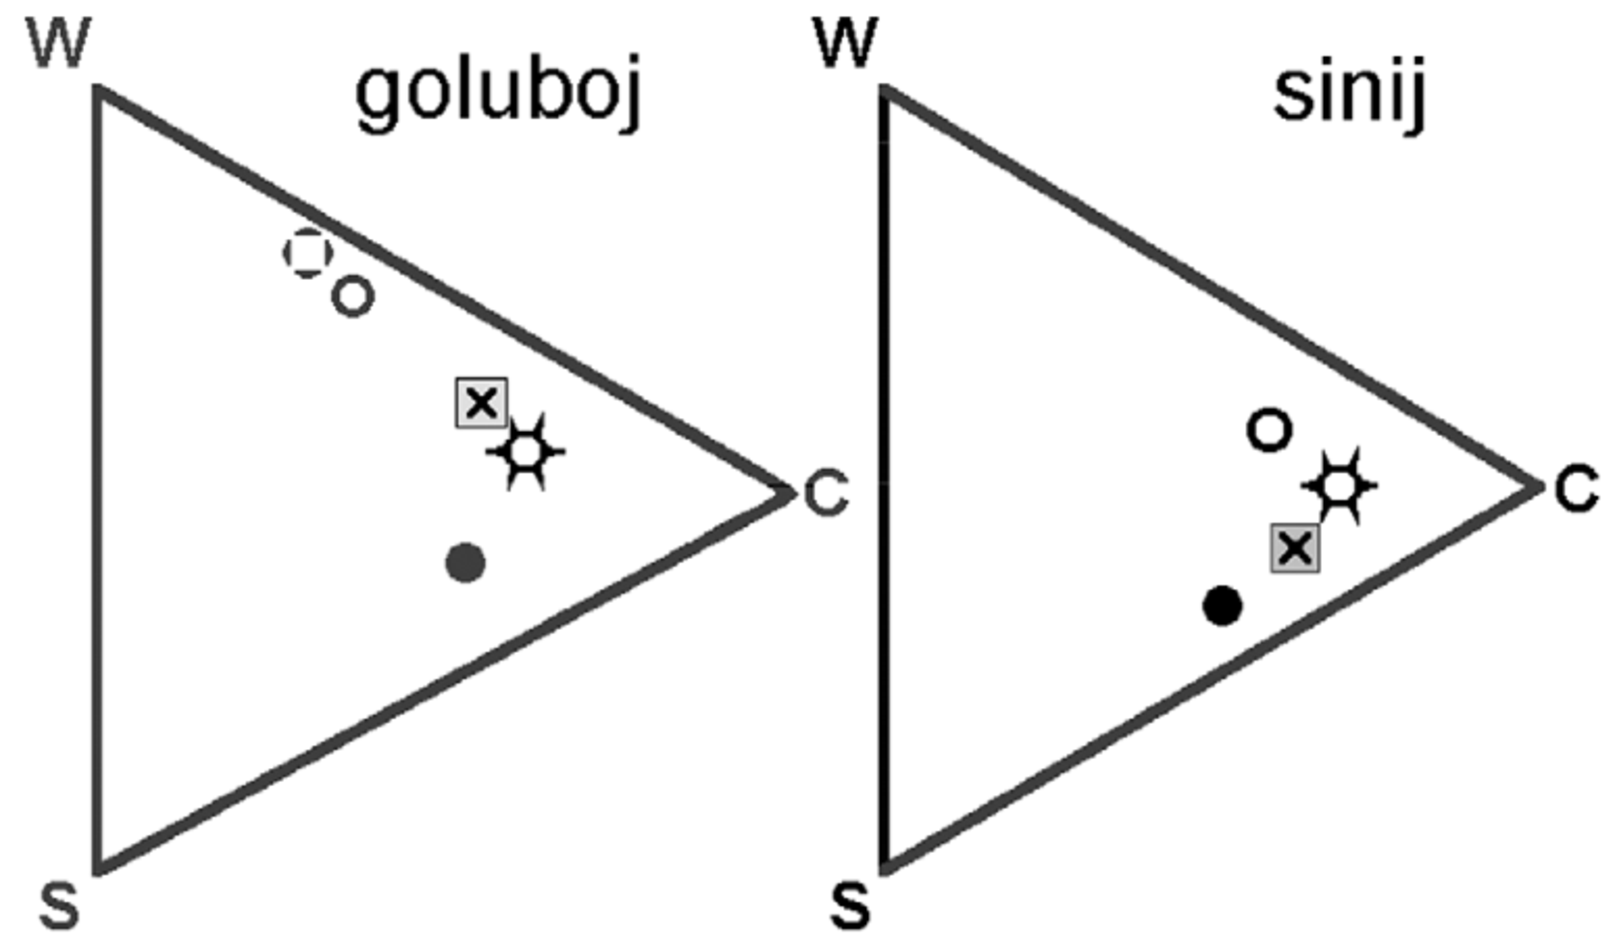
\includegraphics[width=.5\textwidth]{./achromatic/figures/russian-diagram.pdf}
  \caption[Location of modified basic colour foci in Russian]{Location
    of modified basic colour foci in Russian projected into the NCS
    blackness-chromaticity triangle. \textit{t\"emno-} `dark' (solid
    circle), \textit{jarko-} `bright' (sun), \textit{svetlo-} `light'
    (open circle) and \textit{bledno-} `pale' (dashed circle). Figure
    from \cite{paramei05singing}.}
  \label{f:ams-russian-diagram}
\end{figure}

\section{Related research}

The suggestions made in the literature about how to implement the
combination of a basic modifier and a basic colour category are
similar to those reported for the category combination strategy
(see \sectref{s:ccs-related-research}) as the basic
  modification strategy could be thought of as a special case of that
strategy.

The process of mapping a set of properties to a specific category can
not be seen as a straightforward overwriting of a specific property
in the base category. For example, a light brown sample is still
darker than a dark yellow sample. So instead of overwriting the
lightness value of the base category with an absolute value, the
modifiers alter the values specified by the base category. As a
result, basic modifiers are relative to the base category they
modify.

Alternatively, the semantics of a combination of a basic
modifier and a basic colour category could be thought of as a context
dependent filtering operation. First, all entities that are categorised
as the basic colour category would be selected from the context. Next,
the average lightness value of the remaining entities could be used to
decide which entity should be named ``dark'' and which should be named
``light''. Although this could be a productive strategy, using  average lightness
values of the remaining entities might yield unwanted results. For example, 
if the contexts would consist for example of
only two very light green colour samples, it would be unlikely one would
be called ``light green'' and the other one ``dark green''. Moreover,
human subjects are able to assign prototypical colour samples to each
description independent of the context in which the colour samples are
presented \citep{safuanova07russian}.

\section{Semantic template}
\is{semantic template!for basic modification strategy}

I hypothesise that the agents maintain different sets of categories,
which each specify a mutual exclusivity relation between its
members. One such set is the set of basic colour categories. For
example, a colour can not at the same time be red and green. A similar
relation holds for the lightness modifiers \textit{light-} and \textit{dark-}:
a colour is considered to be either light or dark and can never be
light and dark at the same time. This relation is represented by
organising colour categories in different sets. Another set of
categories could be those that specify the chromaticity of a
particular colour, like \textit{pale-} and \textit{bright-}.

The approach of agents maintaining several category sets, ensures a
uniform treatment of each of these sets in all of the strategies
introduced before. This allows for example to only specify some \enlargethispage{\baselineskip}
dimensions of a colour sample, as in \textit{bright green}, or to specify
graded membership, as in \textit{darkish red}.

As I am still pursuing a compositional semantics, I will start from
the semantics of the category combination strategy, as this is
already quite similar to the semantics needed for the current
strategy. The transformation proposed for that strategy can not be
applied anymore, as the modifier category is not a member of the basic
colour category set.

The transformation I propose, shifts the modifiers to the borders
defined by the other basic colour categories. So for example, let us
suppose the base category is yellow. The light modifier will now be
shifted to the border with the white category and the dark modifier to
the border with the brown category. A schematic representation of this
operation is shown in \figref{f:ams-semantics-schematic}.

\begin{figure}
\centering
\subfigure[]{
  
\includegraphics[width=.3\textwidth]{./achromatic/figures/semantics-achromatic.pdf}
  \label{f:ams-semantics-basic}
}
\subfigure[]{
  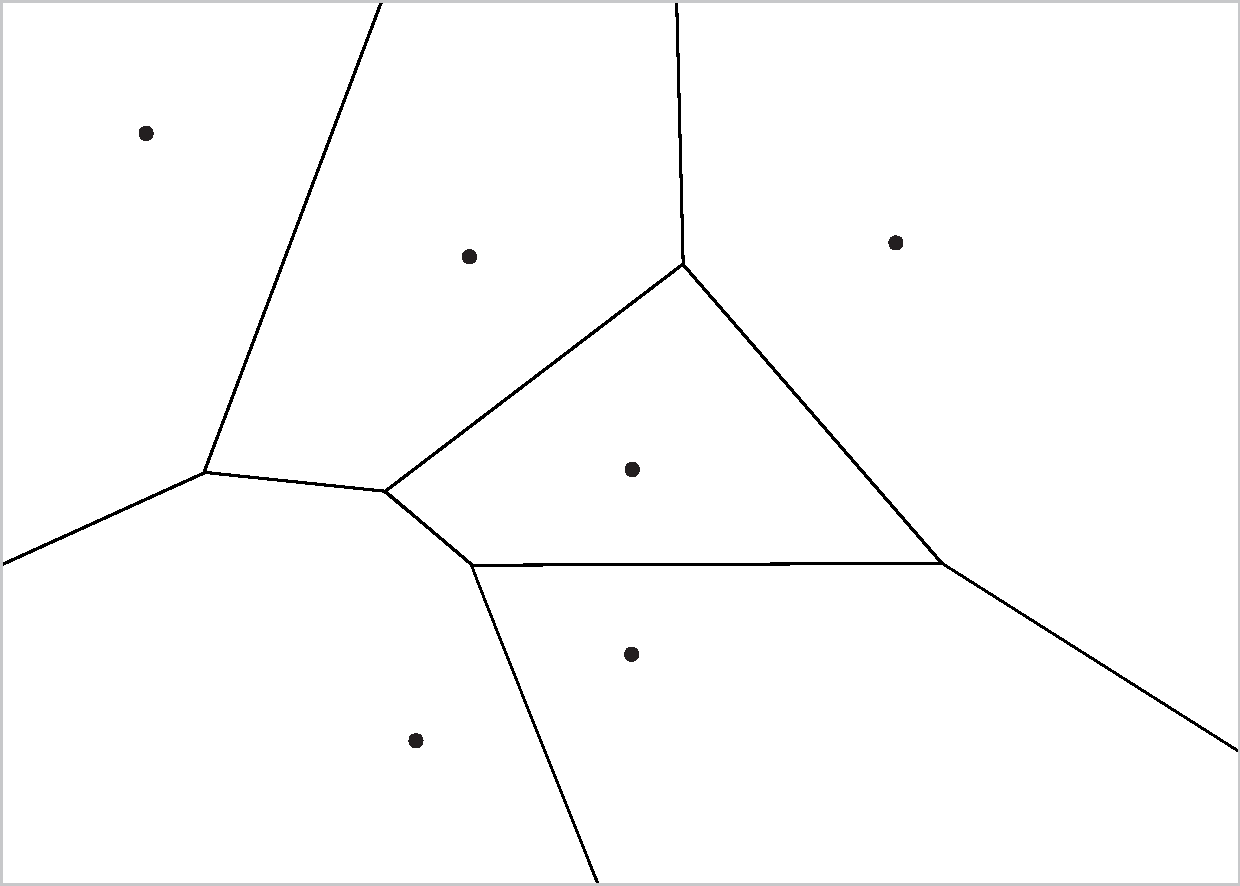
\includegraphics[width=.3\textwidth]{./achromatic/figures/semantics-basic-categories.pdf}
  \label{f:ams-semantics-basic-categories}
}
\subfigure[]{
  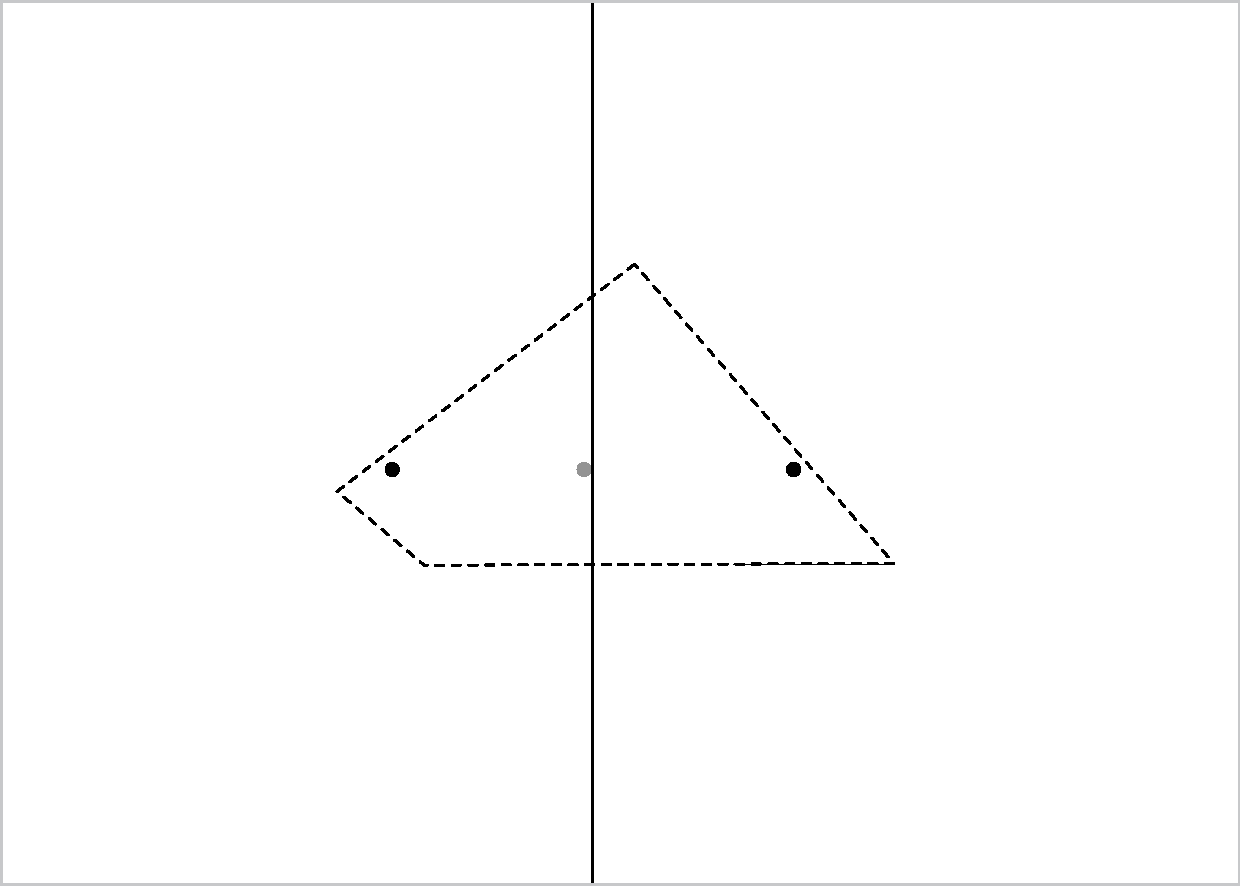
\includegraphics[width=.3\textwidth]{./achromatic/figures/semantics-achromatic-transformed.pdf}
  \label{f:ams-semantics-basic-transformed}
}
\caption[Schematic representation of the transformation for basic
modifiers]{Schematic representation of the transformation for
  basic modifiers: \subref{f:ams-semantics-basic} the
  partitioning of the colour space based on two basic modifiers;
  \subref{f:ams-semantics-basic-categories} the partitioning of the
  colour space based on the basic colour categories;
  \subref{f:ams-semantics-basic-transformed} the transformation
  of the basic modifiers towards one of the basic colour
  categories. The transformed basic modifiers lie on the border
 of the basic colour category.}
\label{f:ams-semantics-schematic}
\end{figure}

The semantics of the basic modification strategy can be
summarised as follows: first a normal categorisation similar to the
one in the basic colour strategy is performed. Before the
basic modifiers are applied, they are transformed corresponding
to the base category that is used during the first categorisation
process. Next the most activated entity is selected from the resulting
set. This process can potentially be extended by a categorisation
process based on activation.

\subsection{Profiling and first categorisation based on colour}

The profiling and the first categorisation process is identical to the
one of the graded membership strategy. It is a strict
implementation of the categorisation process, as in interpretation
only samples that are most similar to the interpreted category are
considered for further processing. This decision is based on the
observation that for basic modifiers, the base category is always
the one that is most similar to the colour sample
\citep{safuanova07russian}.

\subsection{Transformation of set of modifying categories}

Based on the category used during the first categorisation process,
the basic modifiers are transformed in such a way they represent 
the partitioning defined by the basic colour categories. This
operation is based on an iterated estimation procedure in which the
location of the modifier is estimated on the line section between the
modifier and the base category. Each time the new location is
estimated, it is reified as a colour sample that is classified using
the basic colour category set. This procedure stops when the new
location is close to the borders of the base category.

The modifying categories are represented as any other colour category,
but also specify a weight for each dimension representing how
relevant this dimension is. For the lightness modifiers, this would
mean that only the lightness dimension is relevant ($L^*$ in the CIE $L^*a^*b^*$ colour
space). For the chromaticity modifiers, this would be the two hue
dimensions ($a^*$ and $b^*$ in the same colour space). When there are two
categories the resulting coordinates are determined based on these
weights: the lower the weight, the less a particular category
contributes to that dimension.

\subsection{Second categorisation based on modifiers}

Once the modifier categories are transformed, they are used for a
second categorisation process. Like in the category combination
  strategy the membership value of the first categorisation process
is overwritten by the one resulting from the second categorisation
process for similar reasons. A ``light-brown'' colour sample could
have a low membership for the base category brown, but might be a very
good member of the light modifier after it is transformed for
brown. This second categorisation process allows the agent to further
specify the subregion of the conceptual space that was classified as
the base category.

\subsection{Optional categorisation based on membership}

An optional categorisation process based on membership can be added to
the process, which allows for a further specification of the subregion
of the colour space. This additional process allows to describe
samples as ``darkish green'' or ``very light yellow'' and could be
added when the subsequent categorisation process is not sufficient to
discriminate a particular colour sample in a context.

\subsection{Selection based on activation}

The selection is based on the membership value that can be altered by
each of the categorisation processes. The entity with the highest
activation is selected as the entity resulting from the complete
process.

\subsection{Semantic constraint network}

\begin{figure}[b]
  \centering
  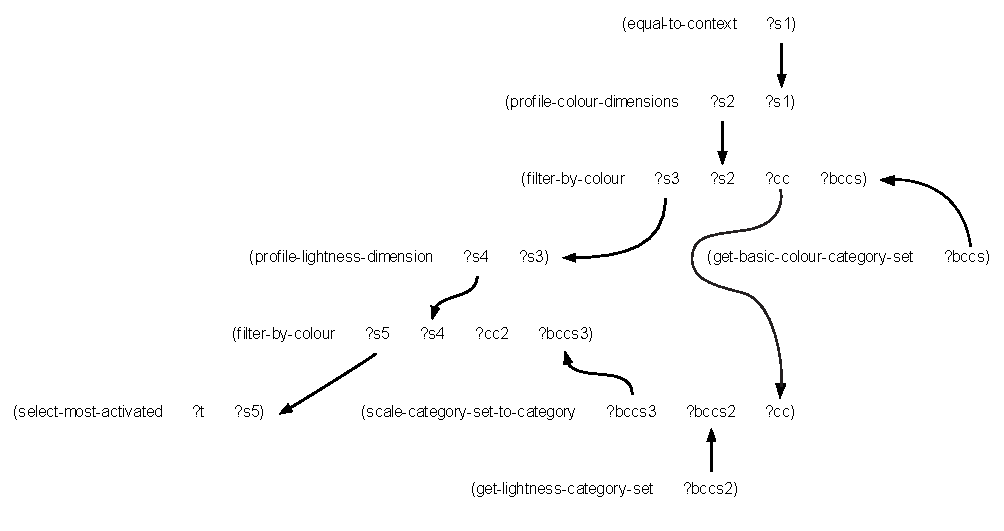
\includegraphics[width=\textwidth]{./achromatic/figures/semantic-program.pdf}
  \caption[Semantic constraint network for basic
  modifiers]{Semantic constraint network for basic modifiers. The
    network consists of two \textsc{Filter-by-Colour} primitives. The
    first uses the basic colour category set, the second the
    lightness modifiers which are transformed into the category used
    by the first categorisation process. This transformation is
    computed by the \textsc{Scale-Category-Set-to-Category}
    primitive.}
  \label{f:ams-semantic-structure}
\end{figure}

The complete semantic network for the basic modification
  strategy is shown in \figref{f:ams-semantic-structure}. It is
very similar to the one for the category combination
  strategy. The first categorisation process based on the basic
colour category set is entirely identical. The
\textsc{Get-Lightness-Category-Set} retrieves the lightness
modifiers known to the agent. The
\textsc{Scale-Category-Set-to-Category} transforms this category set
to the category that was used during the first categorisation
process. The resulting category set is used by the second
\textsc{Filter-by-Colour} operation. Finally,
\textsc{Select-Most-Activated} returns the entity with the highest
entity from the resulting set. An optional
\textsc{Filter-by-Membership} primitive can be added between the last
two primitives.



\subsection{Semantic primitives}

\definition{Semantic primitive}{Get-Lightness-Colour-Category-Set}

\begin{explanation}{description}
  Retrieves all lightness known by the agent.
\end{explanation}

\begin{explanation}{slots}
  \verb+?colour-category-set+ (of type category-set)
\end{explanation}

\begin{explanation}{revision specs}
  $\emptyset$: collects all lightness modifiers known to the agent
  and binds it to \verb+?colour-category-set+
\end{explanation}

\definition{Semantic primitive}{Scale-Category-Set-to-Category}

\begin{explanation}{description}
  Scales all categories in a category set so that they fit into a
  specific category. The borders of that category are determined by
  the other categories in the category set to which that category
  belongs. The category does not need to be a member of the category
  set that is transformed, but the categories of both sets should be
  compatible so they can be successfully combined, like for example
  scaling a set of colour categories to another colour category from
  another category set.
\end{explanation}

\begin{explanation}{slots}
  \verb+?transformed-category-set+ of type \emph{category-set} \\
  \verb+?category-set+ of type \emph{category-set} \\
  \verb+?category+ of type \emph{colour-category}
\end{explanation}

\begin{explanation}{revision specs}
  \verb+?category ?category-set+: scales all categories in the category
  set towards \verb+?category+ bound to \verb+?category+ so that they
  are on the border of \verb+?category+
\end{explanation}

\section{Syntactic templates}

The templates introduced in the previous chapter can be used to cover
each part of the semantic constraint network in \figref{f:ams-semantic-structure}. The linguistic structure for
\textit{t\"emno-rozovyj} is shown in \figref{f:ams-linguistic-structure}.

\begin{figure}[htbp]
  \centering
  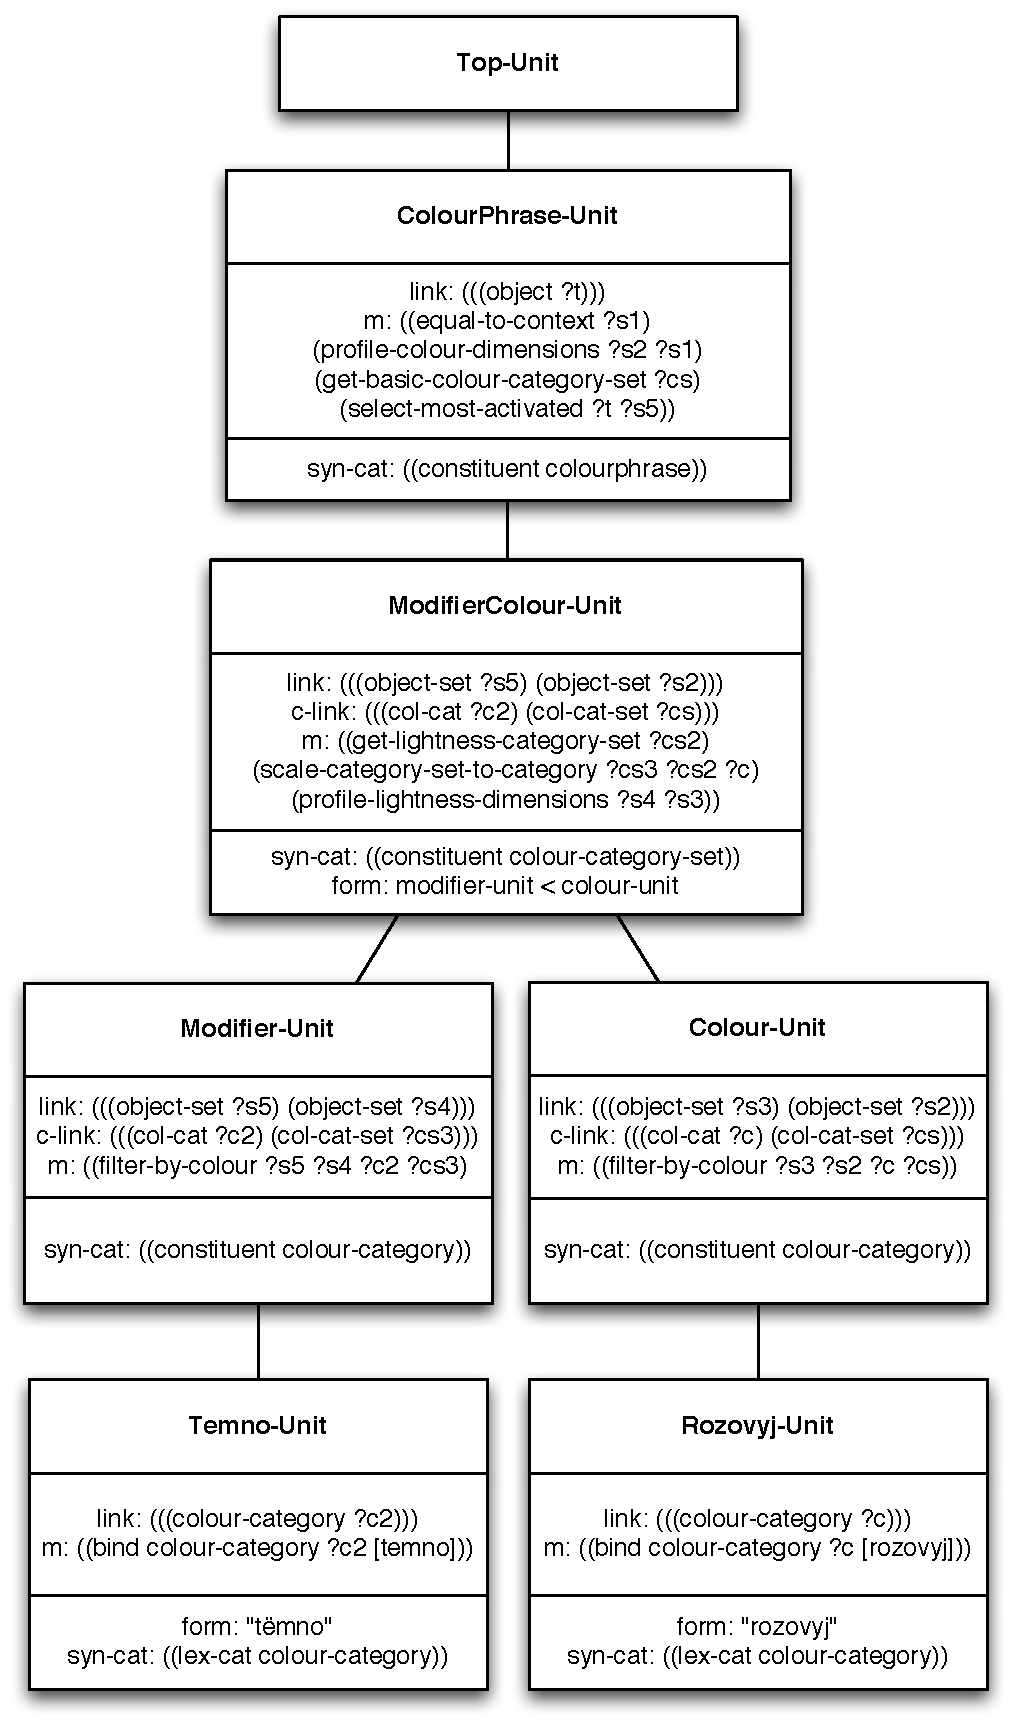
\includegraphics[width=.8\textwidth]{./achromatic/figures/linguistic-structure.pdf}
  \caption[Linguistic structure for basic modifiers]{Linguistic
    structure for basic modifiers. The structure is similar to the
    one presented in the previous chapter, but with a different
    instantiated rule based of Syntactic template 2.1 that introduces
    the ModifierColour unit to the structure.}
  \label{f:ams-linguistic-structure}
\end{figure}

\subsection*{Syntactic template 2.2: Re-use of constructions}
\is{syntactic template!re-use of constructions}

The syntactic template 2.2 that was introduced in the previous chapter
can also be used to express the parts of the basic
  modification strategy that are not yet covered by any of the other
rules. It encapsulates all remaining primitives t and takes care of
all the needed variable equalities between its subunits and the
contextual rule of the basic colour strategy. It is responsible for
introducing the ModifierColour-unit in \figref{f:ams-linguistic-structure} in both producing and parsing.

\footnotesize
\ltitle{ModifierColour rule}
\begin{lstlisting}
((?top-unit
  (sem-subunits (?modifier-unit ?colour-unit))
  (tag ?meaning
       (meaning ((scale-category-set-to-category ?cs3 ?cs2 ?cc)
                 (get-lightness-category-set ?cs2)
                 (profile-lightness-dimensions ?s3 ?s2)))))
 (?modifier-unit
  (link (((entity-set ?s4) (entity-set ?s3))))
  (c-link (((colour-category ?cc2) (colour-category-set ?cs3)))))
 (?colour-unit
  (link (((entity-set ?s2) (entity-set ?s1))))
  (c-link (((colour-category ?cc) (colour-category-set ?cs)))))
 ((J ?modifiercolour-unit ?top-unit (?modifier-unit ?colour-unit))
  ?meaning
  (link (((entity-set ?s4) (entity-set ?s1))))
  (c-link (((colour-category ?cc2) (colour-category-set ?cs))))))
<-->
((?top-unit
  (syn-subunits (?modifier-unit ?colour-unit))
  (tag ?form 
       (form ((meets ?modifier-unit ?colour-unit)))))
 (?modifier-unit 
  (syn-cat ((constituent colour-category))))
 (?colour-unit 
  (syn-cat ((constituent colour-category))))
 ((J ?modifiercolour-unit ?top-unit (?modifier-unit ?colour-unit))
  ?form
  (syn-cat ((constituent colour-category)))))
\end{lstlisting}
\normalsize

\section{Baseline Experiment}
\is{baseline experiment!for basic modification strategy}

The baseline experiment will compare three different predefined language
systems. Each of them is based on the Russian colour category system
\citep{safuanova07russian}. The first one is based on the strict
version of the basic colour strategy. The second one is based
on the basic modification strategy using 2 basic
modifiers: \textit{svleto} (`light') and \textit{t\"emno} (`dark'). The modifiers
are specified as maximal and minimal lightness values and are only
specified in the lightness dimension. The third language system is
based on the basic modification strategy which includes a
categorisation process based on membership using the same basic
semantic entities.

The foci of the basic and modified colour categories have been
reported in the Natural Color System \citep{safuanova07russian} and
have been converted using the method described in Appendix
\ref{s:NCS}. The resulting foci are shown in \figref{f:ams-russian-basic-modifiers}.

\begin{figure}[htpb]
  \centering
  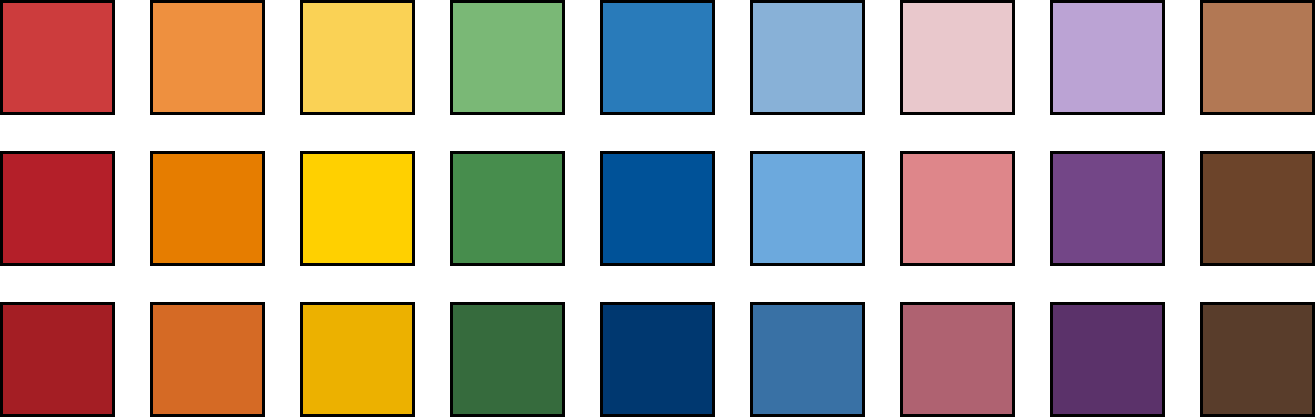
\includegraphics[height=3.75cm]{./achromatic/figures/russian-modified-foci.pdf}
  \caption[Foci of modified basic colour categories in Russian]{Foci
    of modified basic colour categories in Russian. The basic colour
    categories are shown in the middle. The top row shows these
    categories modified with \textit{svleto-} `light' and the bottom
    row shows the same categories modified with \textit{t\"emno-}
    `dark'.  From left to right: \textit{krasnij} `red', \textit{oran\v
    zevyj} `orange', \textit{\v z\"eltij} `yellow',
    \textit{zel\"enyj} `green', \textit{sinij} `dark blue',
    \textit{goluboj} `light blue', \textit{rozovyj} `rose',
    \textit{fioletovyj} `purple' and \textit{kori\v cnevyj} `brown'.}
  \label{f:ams-russian-basic-modifiers}
\end{figure}

As a first test of the proposed semantics, I run a naming benchmark
over all the colour chips reported in the study (shown in \figref{f:ams-russian-basic-modifiers})
\is{naming benchmark!for basic modification strategy}. 
I run the production
procedure and compare the resulting names to the ones reported by the
study. The results for this benchmark are quite good: 15 out of 18
modified chips are named correctly. The chips that were named
incorrectly are shown in \tabref{t:ams-russian-naming-benchmark}

\begin{table}[htpb]
  \centering
  \begin{tabular}{>{\itshape}l>{\itshape}l}
  \lsptoprule
    \normalfont expected name & \normalfont produced name \\
    \midrule
    t\"emno-\v z\"eltij & \normalfont -- \\
    t\"emno-goluboj & svleto-sinij \\
    svleto-sinij & t\"emno-goluboj\\
    \lspbottomrule
  \end{tabular}
  \caption[Naming benchmark for Russian lightness modifiers]{Naming benchmark for Russian lightness modifiers. Only the three samples that were named incorrectly are shown.}
  \label{t:ams-russian-naming-benchmark}
\end{table}

\textit{t\"emno-\v z\"eltij} could not be
named, as it is still considered a light shade of yellow. The names
for the colours samples for \textit{t\"emno-goluboj} (`dark light blue')
and \textit{svleto-sinij} (`light dark blue') were mixed up, as the former
is lighter than the second, which is also reported in literature
\citep{safuanova07russian}. All other colour samples were named
correctly.

\subsection*{Results}

The results of the baseline experiment are shown in \figref{f:ams-baseline}. The language system in which agents can use
basic modifiers reaches a higher level of baseline communicative
success when compared to the basic colour strategy. This
positive impact is even higher when agents are allowed to grade the
resulting membership (compare results of basic modifiers to
graded basic modifiers). The higher the expressivity of the
agents, the higher the resulting baseline communicative success.

When compared to the baseline experiment of the category
  combination strategy, the resulting baseline communicative success
is slightly lower. This is probably due to the lower number of
categories that can be used to modify the basic categorisation
process. In the current experiment, only two such categories are
present, whereas in the category combination experiment, all
adjacent colour categories could be used.

\begin{figure}[htpb]
  \centering
  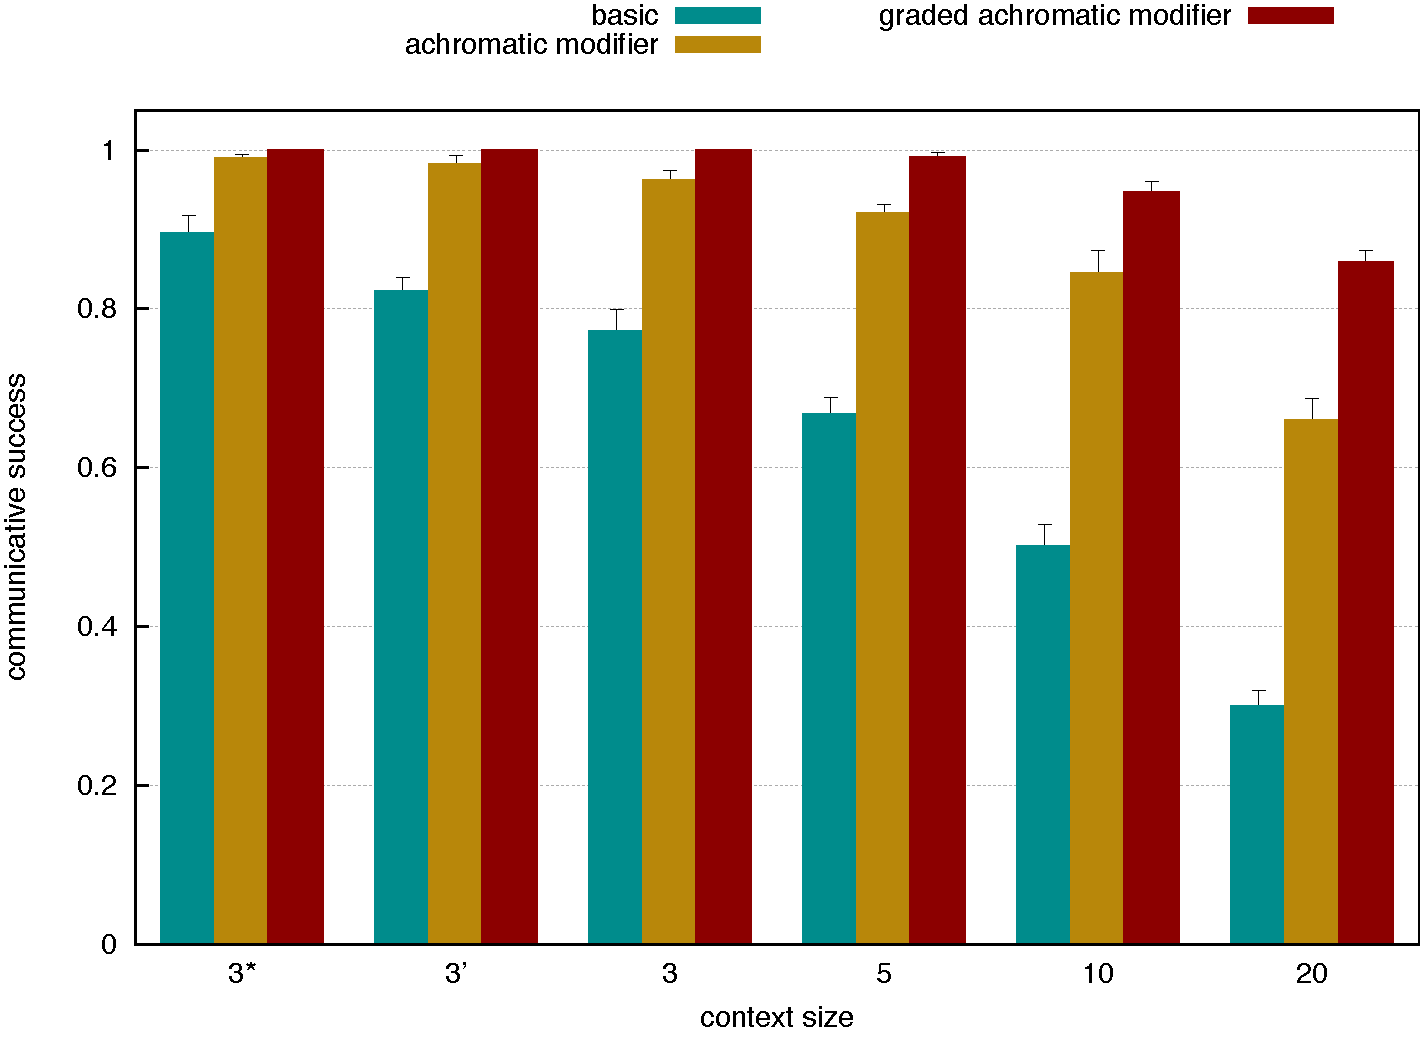
\includegraphics[width=.8\textwidth]{./achromatic/figures/baseline.pdf}
  \caption[Baseline communicative success for basic modification
  strategy]{Baseline communicative success for basic modification
    strategy. The baseline success of the basic colour strategy is
    lower than the success of the basic modification strategy. When
    this strategy is extended with a categorisation process based on
    membership, the resulting baseline success is even higher.}
  \label{f:ams-baseline}
\end{figure}

\section{Conclusion}

In this chapter I have proposed a semantic template that allows
agents to use basic modifiers. This template is based on
observations in natural language and is highly compositional. This
compositionality allows agents to re-use the semantic primitives and
constructions that have been introduced in previous chapters.

The proposed semantic template in which the lightness categories are
represented in a set of colour categories separate from the
basic colour categories, allows for the re-use of each of the
previous language strategies using these lightness
categories. Representing the semantics of descriptions like \textit{light}
or \textit{very light} requires the simple replacement of the primitive that
retrieves the colour category set from the ontology of an agent.